%!TEX TS-program = xelatex

%	Author: Dmitry Rodin (d.rod1n1721@gmail.com)
%	

%	Основной документ
\documentclass[a4paper, 14pt]{extarticle}	%	14-й шрифт дл текста

%	Преамбула для оформления файла Latex
%	Преамбула

%	Шрифты

%	Гиперссылки

%	Отступы по ГОСТ

%	Секции без номеров(ВВЕДЕНИЕ, ЗАКЛЮЧЕНИЕ, СОКРАЩЕНИЯ ПРИНЯТЫЕ В ТЕКСТЕ....)
\newcommand{\anonsection}[1]{
	\phantomsection % Корректный переход по ссылкам в содержании
	\paragraph{\centerline{{#1}}\vspace{1.5em}}
	\addcontentsline{toc}{section}{\uppercase{#1}}
}

%	Библиография
\makeatletter
\renewenvironment{thebibliography}[1]
{\section*{\refname}
	\list{\@biblabel{\@arabic\c@enumiv}}
	{\settowidth\labelwidth{\@biblabel{#1}}
		\leftmargin\labelsep
		\itemindent 16.7mm
		\@openbib@code
		\usecounter{enumiv}
		\let\p@enumiv\@empty
		\renewcommand\theenumiv{\@arabic\c@enumiv}
	}
	\setlength{\itemsep}{0pt}
}
\makeatother

%	Начало документа
\begin{document}
	%	Содержание
	\tableofcontents
	\clearpage
	
	%	Сокращения, принятые в тексте
	\anonsection{СОКРАЩЕНИЯ, ПРИНЯТЫЕ В ТЕКСТЕ}

\begin{tabular}{ l l  }
	БСК & блок силовой коммутации \\
	БУК	&	блок усиления и коммутации\\
	БЦВМ &	бортовая цифровая вычислительная машина\\
	БЭ &		блок электроники\\
	ВА &		возвращаемый аппарат\\
	ДДУ &		дискретный датчик угла\\
	ИТ	&	источник тока\\
	НС	&	наблюдатель состояния\\
	ОУ	&	объект управления\\
	ПТДУ &	посадочная твердотопливная двигательная установка\\
	ПТК НП &	пилотируемый транспортный корабль нового поколения \\
	ПУ	&	посадочное устройство\\
	РДТТ	&	ракетный двигатель твердого топлива\\
	РМ	&	рулевая машинка\\
	РП	&	рулевой привод\\
	РПУ	&	релейное пороговое устройство\\
	РС	&	регулятор состояния\\
	СУ	&	система управления\\
	СУБ	&	сопловые управляемые блоки\\
	ТП	&	телеметрический потенциометр\\
	ТРТ	&	твердое ракетное топливо\\
	УПК	&	устройство преобразования кода Грея в двоичный код\\
	УСДК &	устройство сравнения двоичных кодов\\
	ЭД	&	электродвигатель\\
	ЭП	&	электромеханический привод\\
	
\end{tabular}

\clearpage
	
	%	Введение
	%	Введение
\anonsection{Введение}

Целью данного курсового проекта является синтез алгоритма наведения и стабилизации центра масс возвращаемого аппарата. Разработка алгоритмов и программного обеспечения математического моделирования замкнутой системы управления в MatLab. Проведение сравнительного анализа результатов моделирования.


Под синтезом системы автоматического управления понимается направленный расчет, имеющий конечной целью отыскание рациональной структуры системы и установление оптимальных величин параметров ее отдельных звеньев. 

Синтез можно трактовать как инженерную задачу, сводящуюся к такому построению системы, при котором обеспечивается выполнение технических требований к ней. Подразумевается, что из многих возможных решений инженер, проектирующий систему, будет выбирать те, которые являются оптимальными с точки зрения существующих конкретных условий и требований к габаритам, весу, простоте, надежности и т. п.

При инженерном синтезе системы автоматического управления необходимо обеспечить, во-первых, требуемую точность и, во-вторых, приемлемый характер переходных процессов.

Обеспечение приемлемых переходных процессов оказывается почти всегда более трудным вследствие большого числа варьируемых параметров и многозначности решения задачи демпфирования системы. Поэтому существующие инженерные методы часто ограничиваются решением только второй задачи, так как обеспечение требуемой точности может быть достаточно просто сделано на основании использования существующих критериев точности и совершенствования их практически не требуется.

В настоящее время для целей синтеза систем автоматического управления широко используются вычислительные машины, позволяющие производить полное или частичное моделирование проектируемой системы
\clearpage
	
	%	Техническое задание на разработку СУ ПТДУ
	%	Требования технического задания на разработку СУ ПТДУ
\anonsection{ОСНОВНАЯ ЧАСТЬ}
\section{Требования технического задания на разработку СУ ПТДУ}

\begin{enumerate}
	\item Рассматривается схема газосвязанной ПТДУ с регулированием тяги
	
	\item Основные потребные параметры ПТДУ определяются значениями
	\begin{itemize}
		\item Диапазон суммарной тяги $R_{\sum} = 9.0 - 22.0$ тс, при этом предполагается возможность реализации управления тягой по заданным алгоритмам в зависимости от реализованных условий посадки, обусловленных разбросом параметров атмосферы, аэродинамических, массовых, инерционных, центровочных характеристик возвращаемого аппарат, параметров, траектории и др
		\item Суммарный импульс тяги по осям всех сопел $I_{\sum} = 260 \text{тс}*\text{c}$
		\item Максимальное время работы $30$ c.
	\end{itemize}
	\item Рассматривается применение в составе ПТДУ от 8 до 12 сопловых управляющих блоков (СУБ), Каждый СУБ имеет два расходных сопла, одно из которых направлено вдоль продольной оси ВА, второе-под углом (30… 45) грд к поперечной плоскости ВА. Регулирование расхода через каждое сопло осуществляется по командам от систем управления дифференцированно с помощью регулятора механического типа, вал которого кинематически связан с рулевой машинкой по командам управления.
	
	\item Сопла, направленные вдоль продольной оси ВА (сопла первой группы), задействуются на основном участке торможения от момента начала работы ПТДУ и до высоты 40 м, с которой начинается приземный участок торможения. Группа обеспечивает гашение линейной скорости ВА на этом участке, а также управление относительно ЦМ по каналам рысканья и тангажа.
	
	\item Сопла, направленные под углом (30…45) грд к поперечной плоскости ВА (сопла второй группы), введены в состав ПТДУ для минимизации воздействия струй работающей ПТДУ на грунт. Сопла второй группы задействуются на приземном участке, а также для управления по каналам рысканья и тангажа на основном участке (при необходимости) и на приземном.
	
	\item Должна быть проработана целесообразность и, при необходимости, реализация управления по каналу крена средствами ПТДУ при ее работе.
\end{enumerate}
\clearpage

\subsection{Назначение ПТДУ}
Посадочная твердотопливная двигательная установка (ПТДУ) предназначена для снижения скорости возвращаемого орбитального аппарата (ВА) на участке приземления от величин, соответствующих установившейся скорости спуска, до заданных значений к моменту касания земли. При этом должна обеспечиваться возможность реализации управления тягой по заданным алгоритмам в зависимости от реализованных условий посадки по командам системы управления ВА.	

Под участком приземления понимается участок спуска ВА, начинающийся в момент включения ПТДУ и заканчивающийся в момент касания первой опоры посадочного устройства (ПУ) ВА с поверхностью полигона. Приведение ВА на полигон обеспечивается управлением ВА до включения ПТДУ. Под полигоном понимается подготовленная посадочная площадка диаметром несколько км. Включение ПТДУ должно производиться на высоте ~1 км над поверхностью полигона.
\clearpage

\subsection{Общий вид ВА}
\begin{figure}[h]
	\centering
	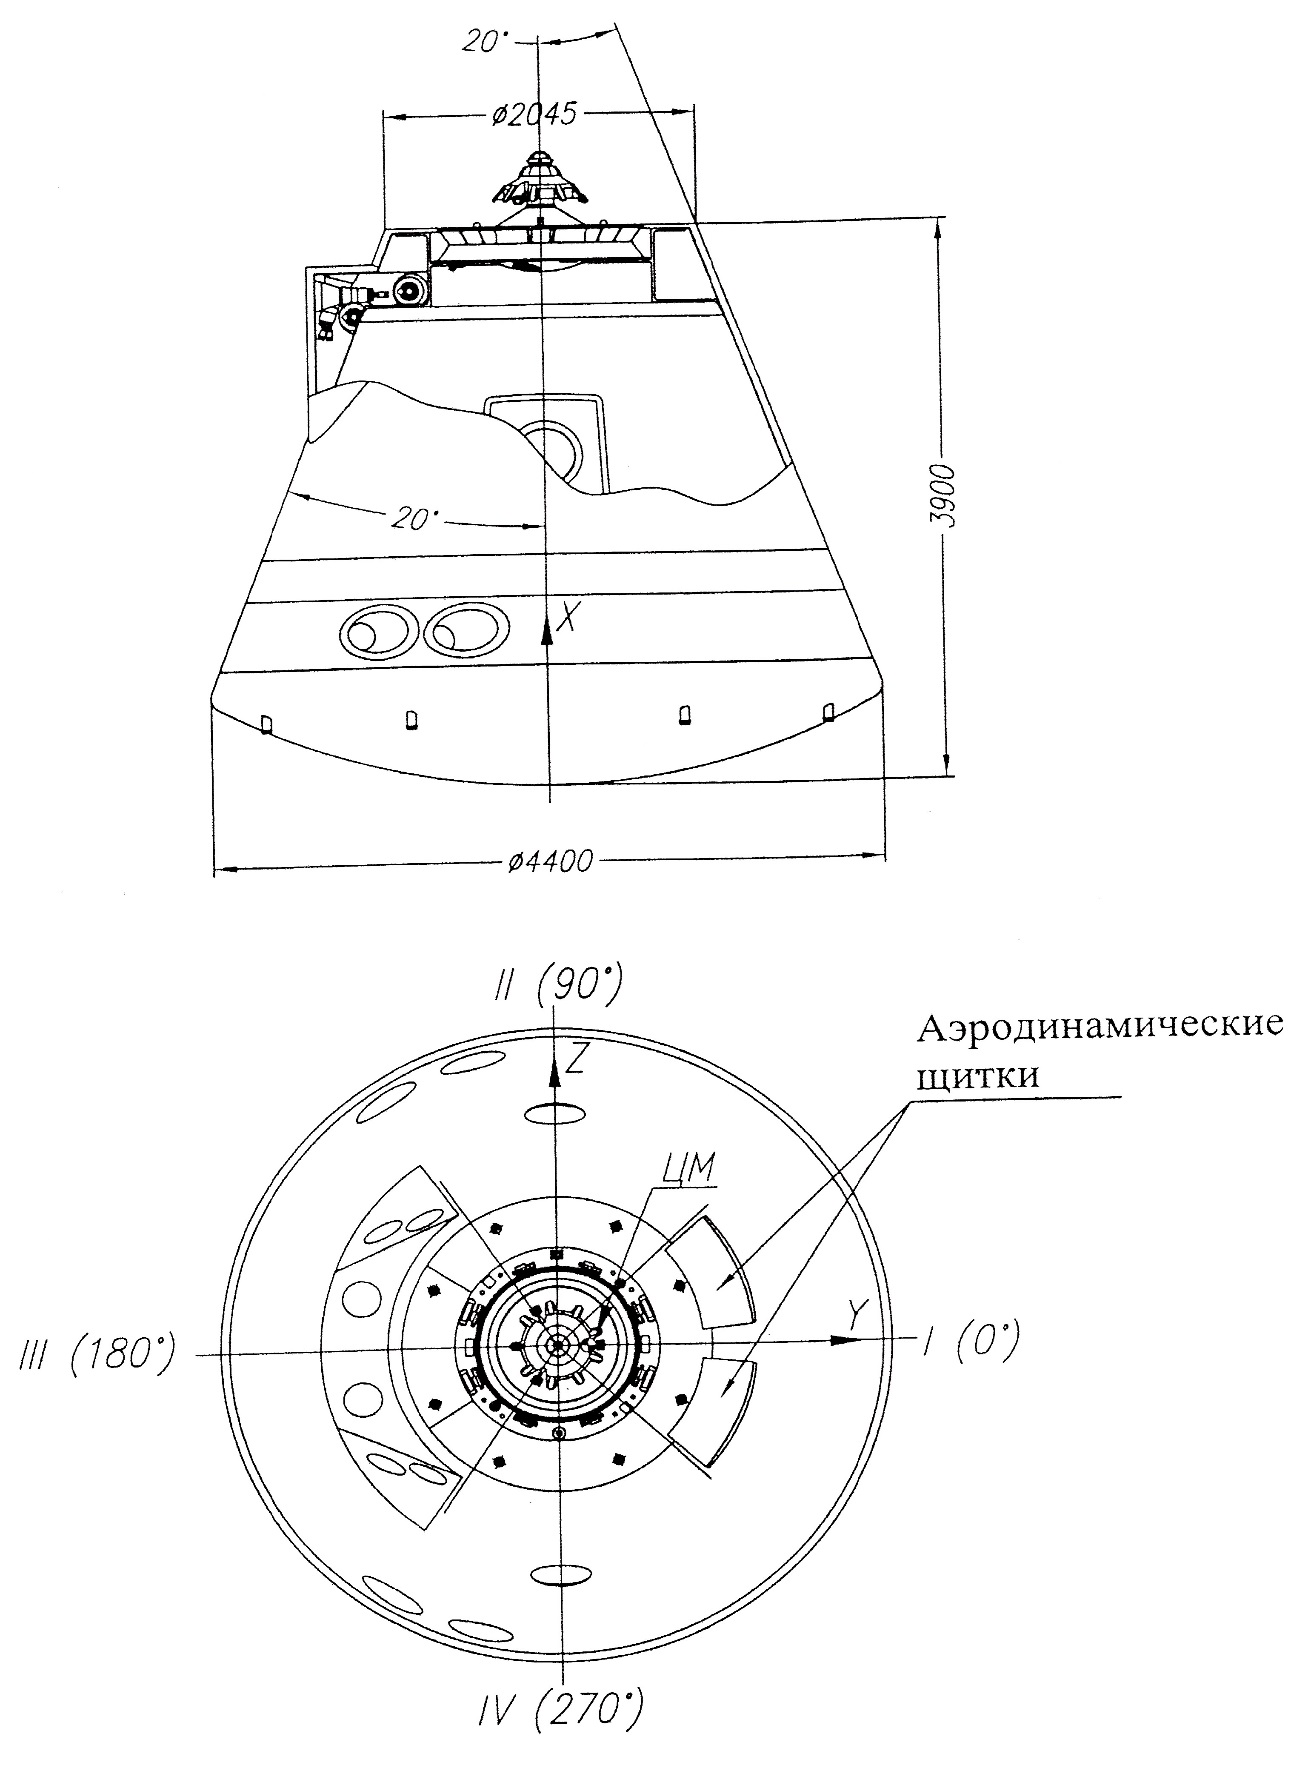
\includegraphics[scale=0.7]{images/va.jpg}
	\caption{Общий вид ВА}
	\label{fig:va_pic}
\end{figure}
\clearpage

\begin{figure}[h]
	\centering
	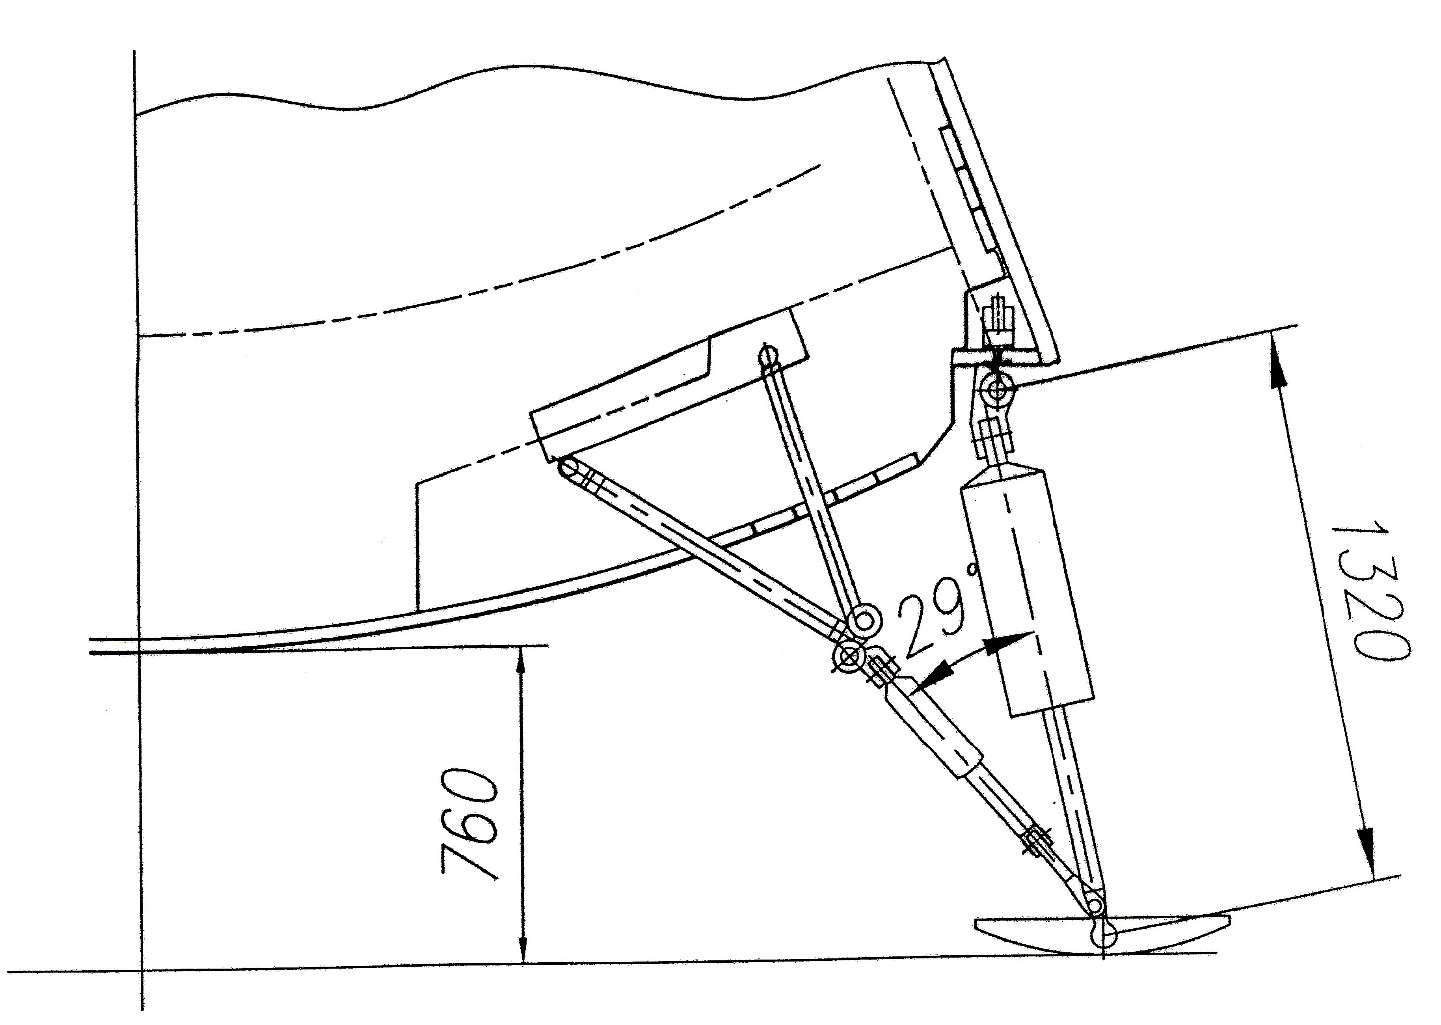
\includegraphics[scale=0.9]{images/posad_config.jpg}
	\caption{Посадочная конфигурация ВА с выпущенным посадочным устройством}
	\label{fig:posad_config}
\end{figure}
\clearpage

\subsection{Конструкция и принцип действия ПТДУ}
ПТДУ представляет собой РДТТ с регулируемой тягой по величине и направлению. На рисунке показана схема ПТДУ. Он состоит из:
\begin{itemize}
	\item двух корпусов типа "кокон"  с наполнителями ТРТ "Г-З"
	\item 16 односопловых управляющих блоков (СУБ)
	\item системы газоходов, газосвязывающего корпуса с наполнителями и СУБ
	\item двух пусковых двигателей 
	\item блока датчиков давления системы измерения давления
	\item рулевого привода (электромеханического или газогидравлического) 
\end{itemize}

Сопла всех СУБ снабжены собственными регуляторами расхода, управляемыми собственными рулевыми машинками. Расположение и маркировка органов управления соответствует рисунку 6.1.

ПТДУ многорежимна. Переход с режима на режим, а также стабилизация давления на любом режиме, обеспечивается изменением газоприхода от поверхности горения за счет изменения скорости горения наполнителя путем кратковременного изменения суммарной площади минимальных сечений сопел.

Создание управляющих сил по каналам тангажа и рыскания на каждом режиме обеспечивается за счет перераспределения расхода продуктов сгорания ТРТ между соплами путем изменения площади минимального сечения каждого сопла при сохранении постоянной суммарной площади минимальных сечений всех сопел:
\begin{equation}
\mu F_{\sum} = \sum_{j=1}^{16} \mu F_j \approx const
\end{equation}
где $\mu F_{\sum}$ - требуемая суммарная эффективная площадь минимальных сечений сопел на соответствующем режиме работы ПТДУ.

$\mu F_j$ - текущая эффективная площадь минимального сечения $j$-го сопла.

При необходимости должна быть обеспечена возможность отсечки тяги ПТДУ по команде СУ. При этом для прекращения горения наполнителей должно выполняться условие:
\begin{equation}
\mu F_{\sum} = \sum_{j=1}^{16} \mu F_j^{max}
\end{equation}
где $\mu F_j^{max}$ - максимальная эффективная площадь минимального сечения $j$ - го сопла.

В случае отказа одного из СУБ или отказа ПМ площадь минимального сечения этого СУБ при дальнешей работе ПТДУ должна оставаться постоянной, при это должна выполняться заданная циклограмма суммарной тяги $R_{\sum}$  и управление остальными СУБ в заданном диапазоне $R$.
\begin{figure}[h]
	\centering
	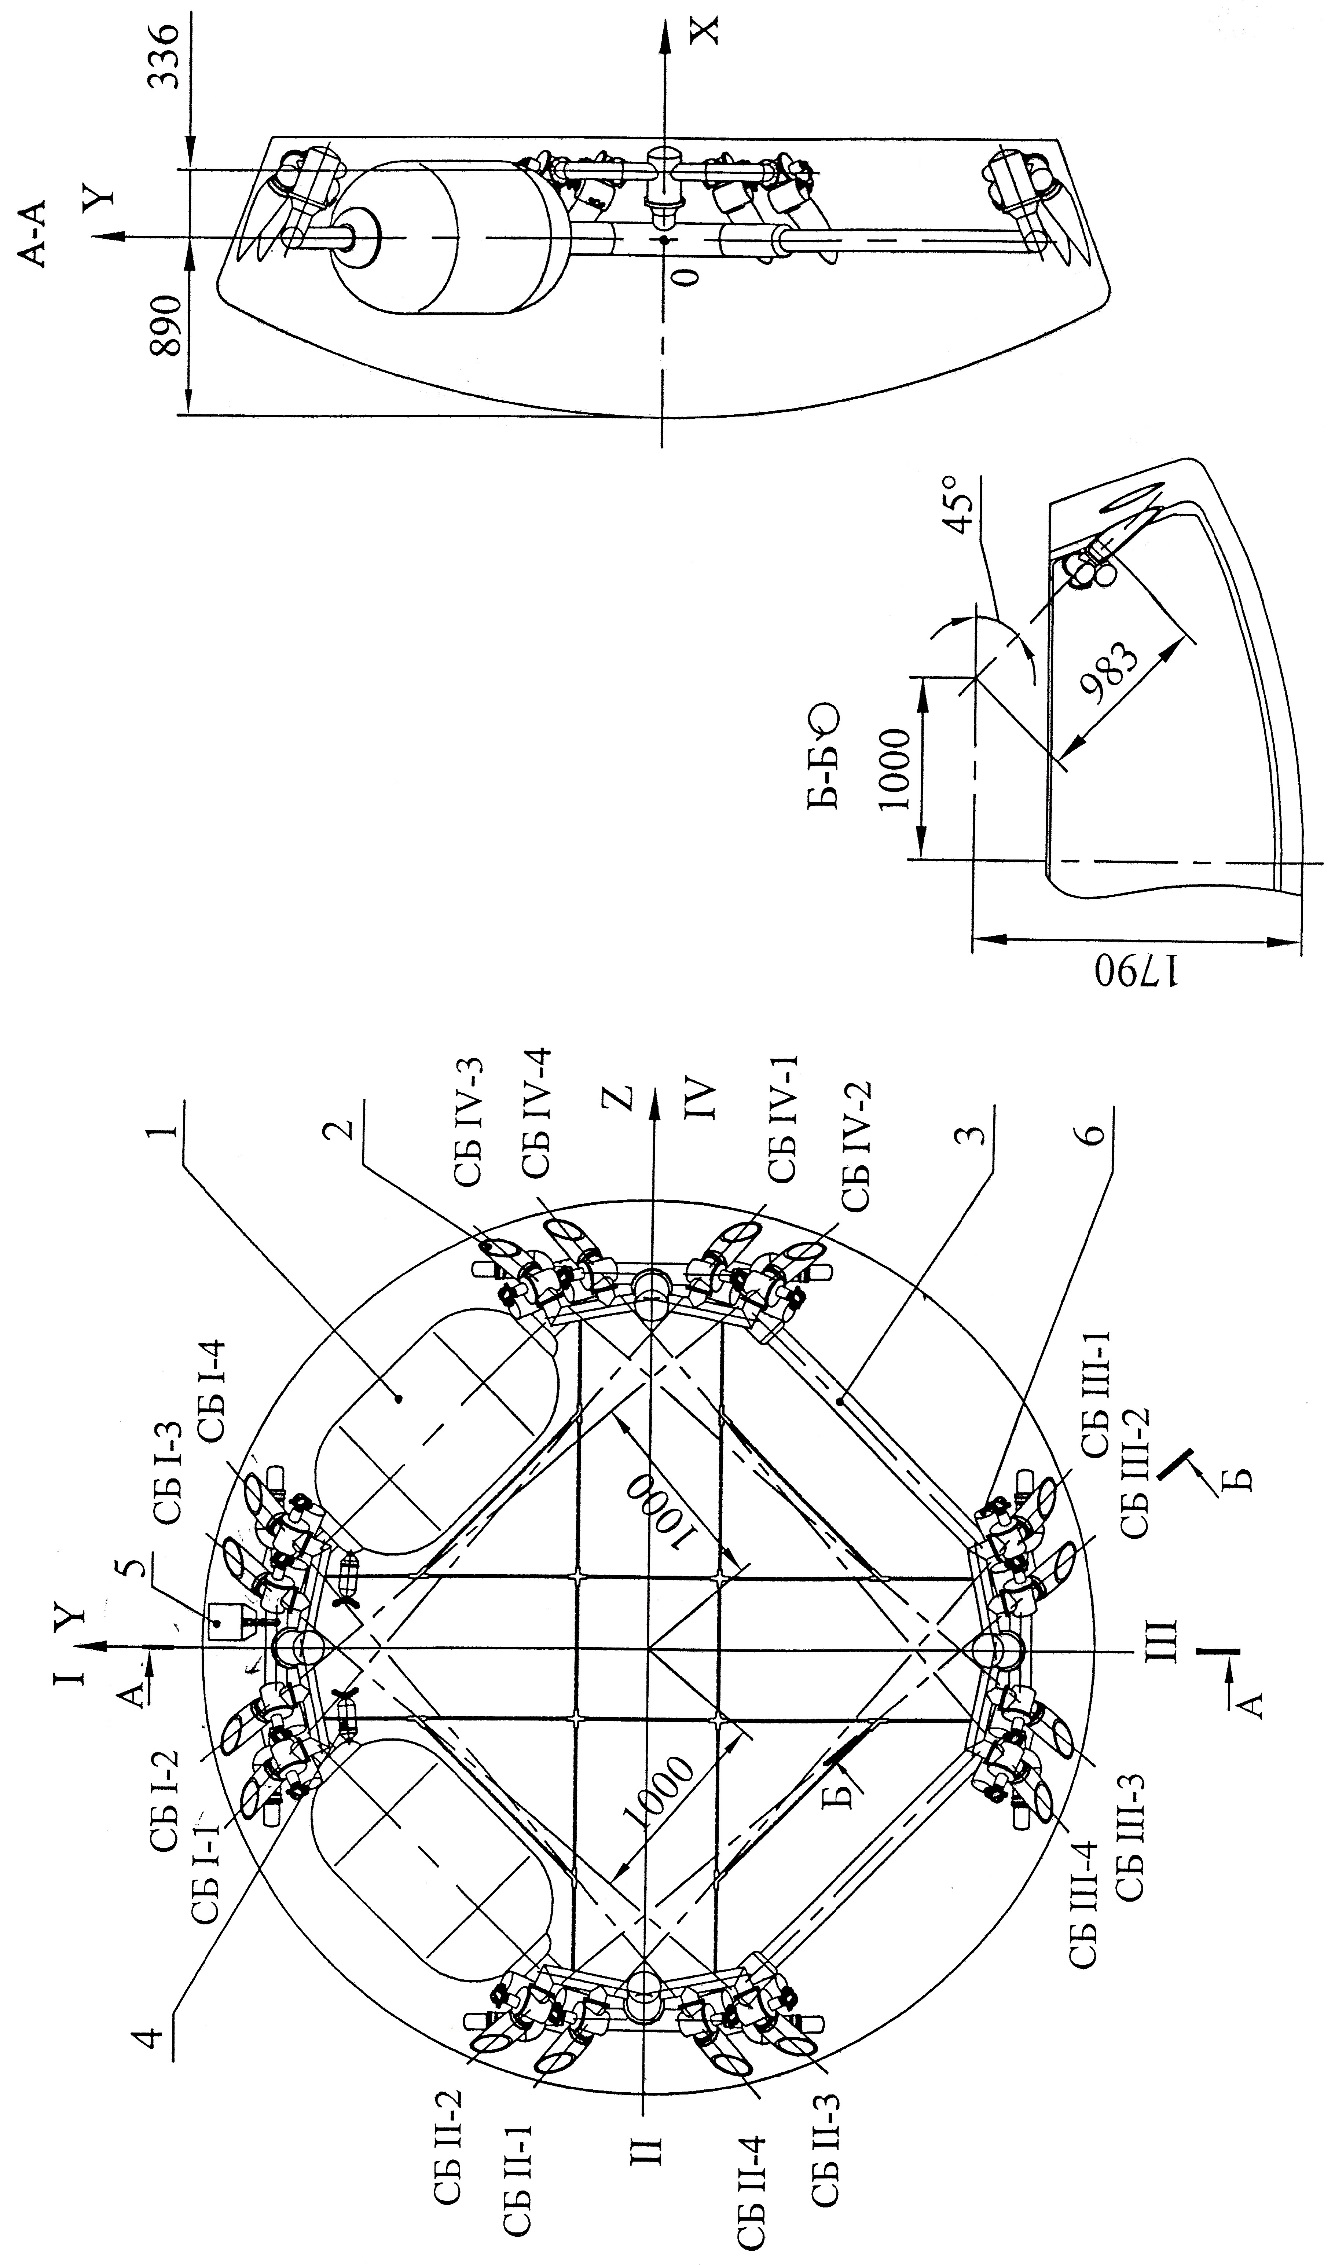
\includegraphics[scale=0.3]{images/scheme_ptdu.jpg}
	\caption{Схема ПТДУ}
	\label{fig:scheme_ptdu}
\end{figure}
\clearpage

\subsection{Характеристики органов управления}

\begin{figure}[h]
	\centering
	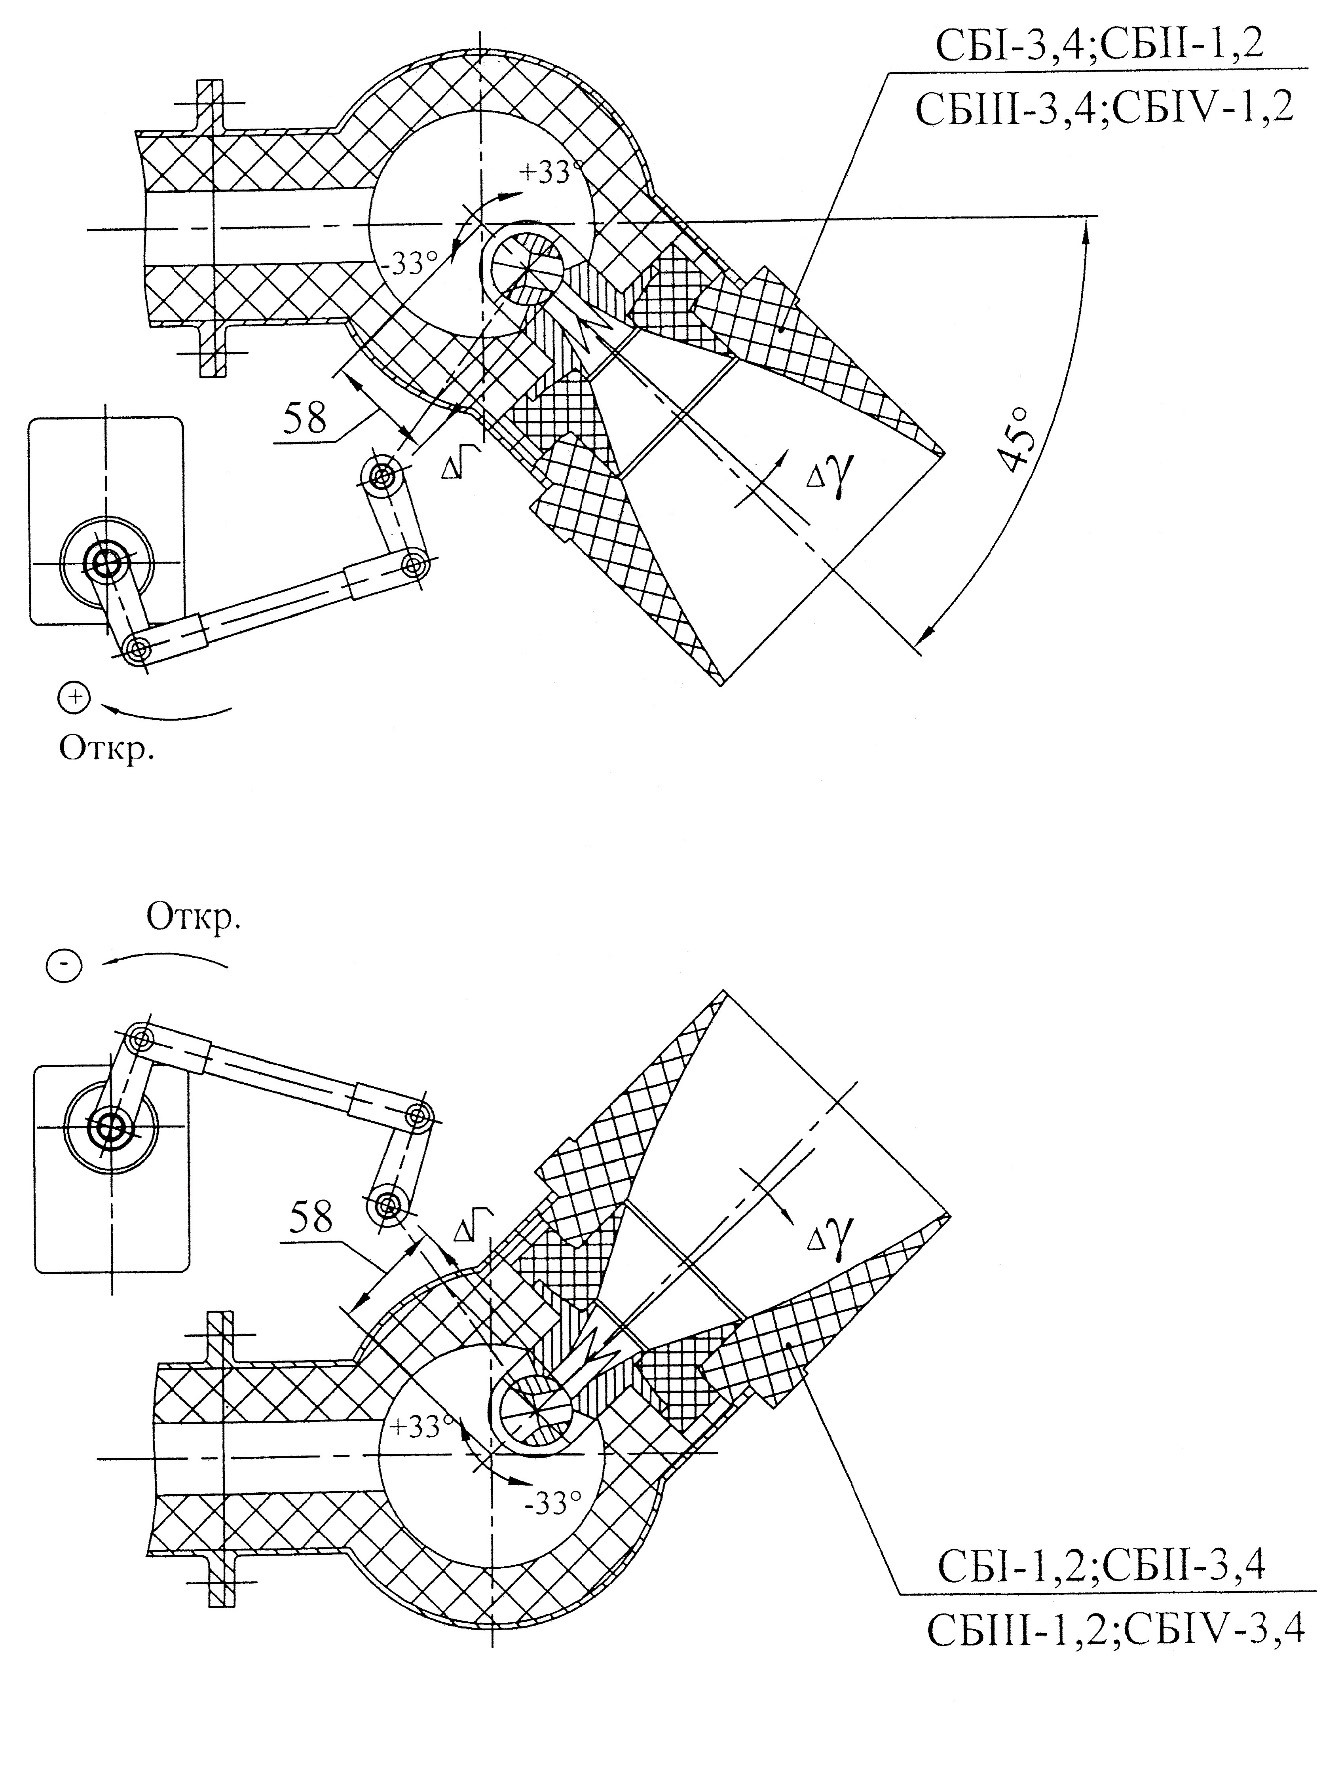
\includegraphics[scale=0.5]{images/scheme_subrp.jpg}
	\caption{Кинематическая схема СУБ с РП}
	\label{fig:scheme_subrp}
\end{figure}

Зависимость эффективной площади минимального сечения единичного сопла СУБ ($\mu F_j$) от угла поворота вала РМ ($\delta_j$ ) представлена на рисунке ~(\ref{fig:effect_nozzle})

\begin{figure}[h]
	\centering
	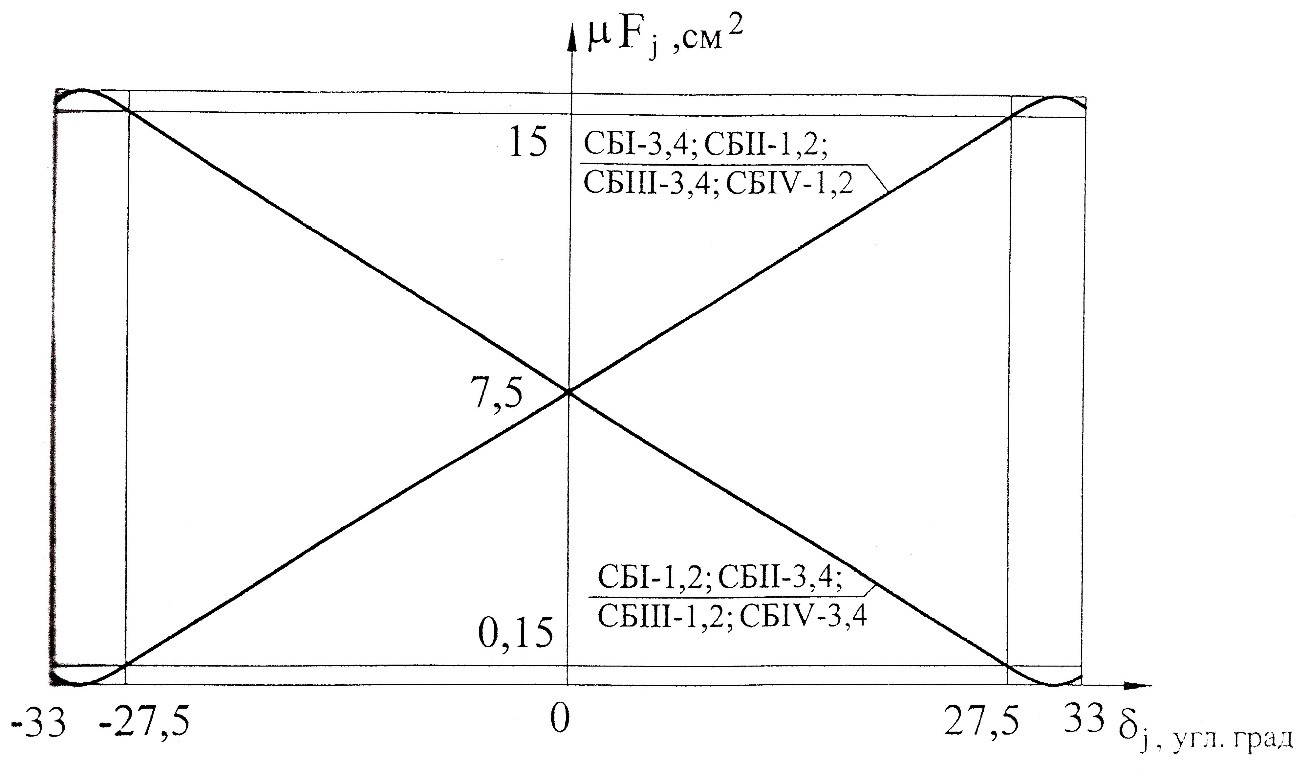
\includegraphics[scale=0.5]{images/effect_nozzle.jpg}
	\caption{Зависимость эффективной площади сечения единичного сопла ($\mu F_j$) от угла поворота вала РМ ($\delta_j$)}
	\label{fig:effect_nozzle}
\end{figure}

При работе ПТДУ используется только линейный участок зависимости $\mu F_j (\delta_j)$.

На участке от $-27.5^{\circ}$ до $27.5^{\circ}$ для данной расходной характеристики допускается линейная аппроксимация:
\begin{equation}
	\label{eq:ur_lin_approxim}
	\delta_j = 3.667 \cdot \mu F_j - 27.5
\end{equation}

Систематическое линейное и угловое отклонение вектора тяги в единичном сопле в зависимости от угла поворота РМ от геометрической оси сопла за счет прямоугольной формы площади минимального сечения регулятора сопла приведено на ~(\ref{fig:effect_nozzle}).

Отклонение происходит в плоскости, проходящей через геометрическую ось сопла перпендикулярно продольной оси корпуса СУБ.

Случайное отклонение вектора тяги от номинального положения геометрической оси сопла в плоскости минимального сечения составляет: линейное $1.5$ мм, угловое $1.5^{\circ}$.

\begin{figure}[h]
	\centering
	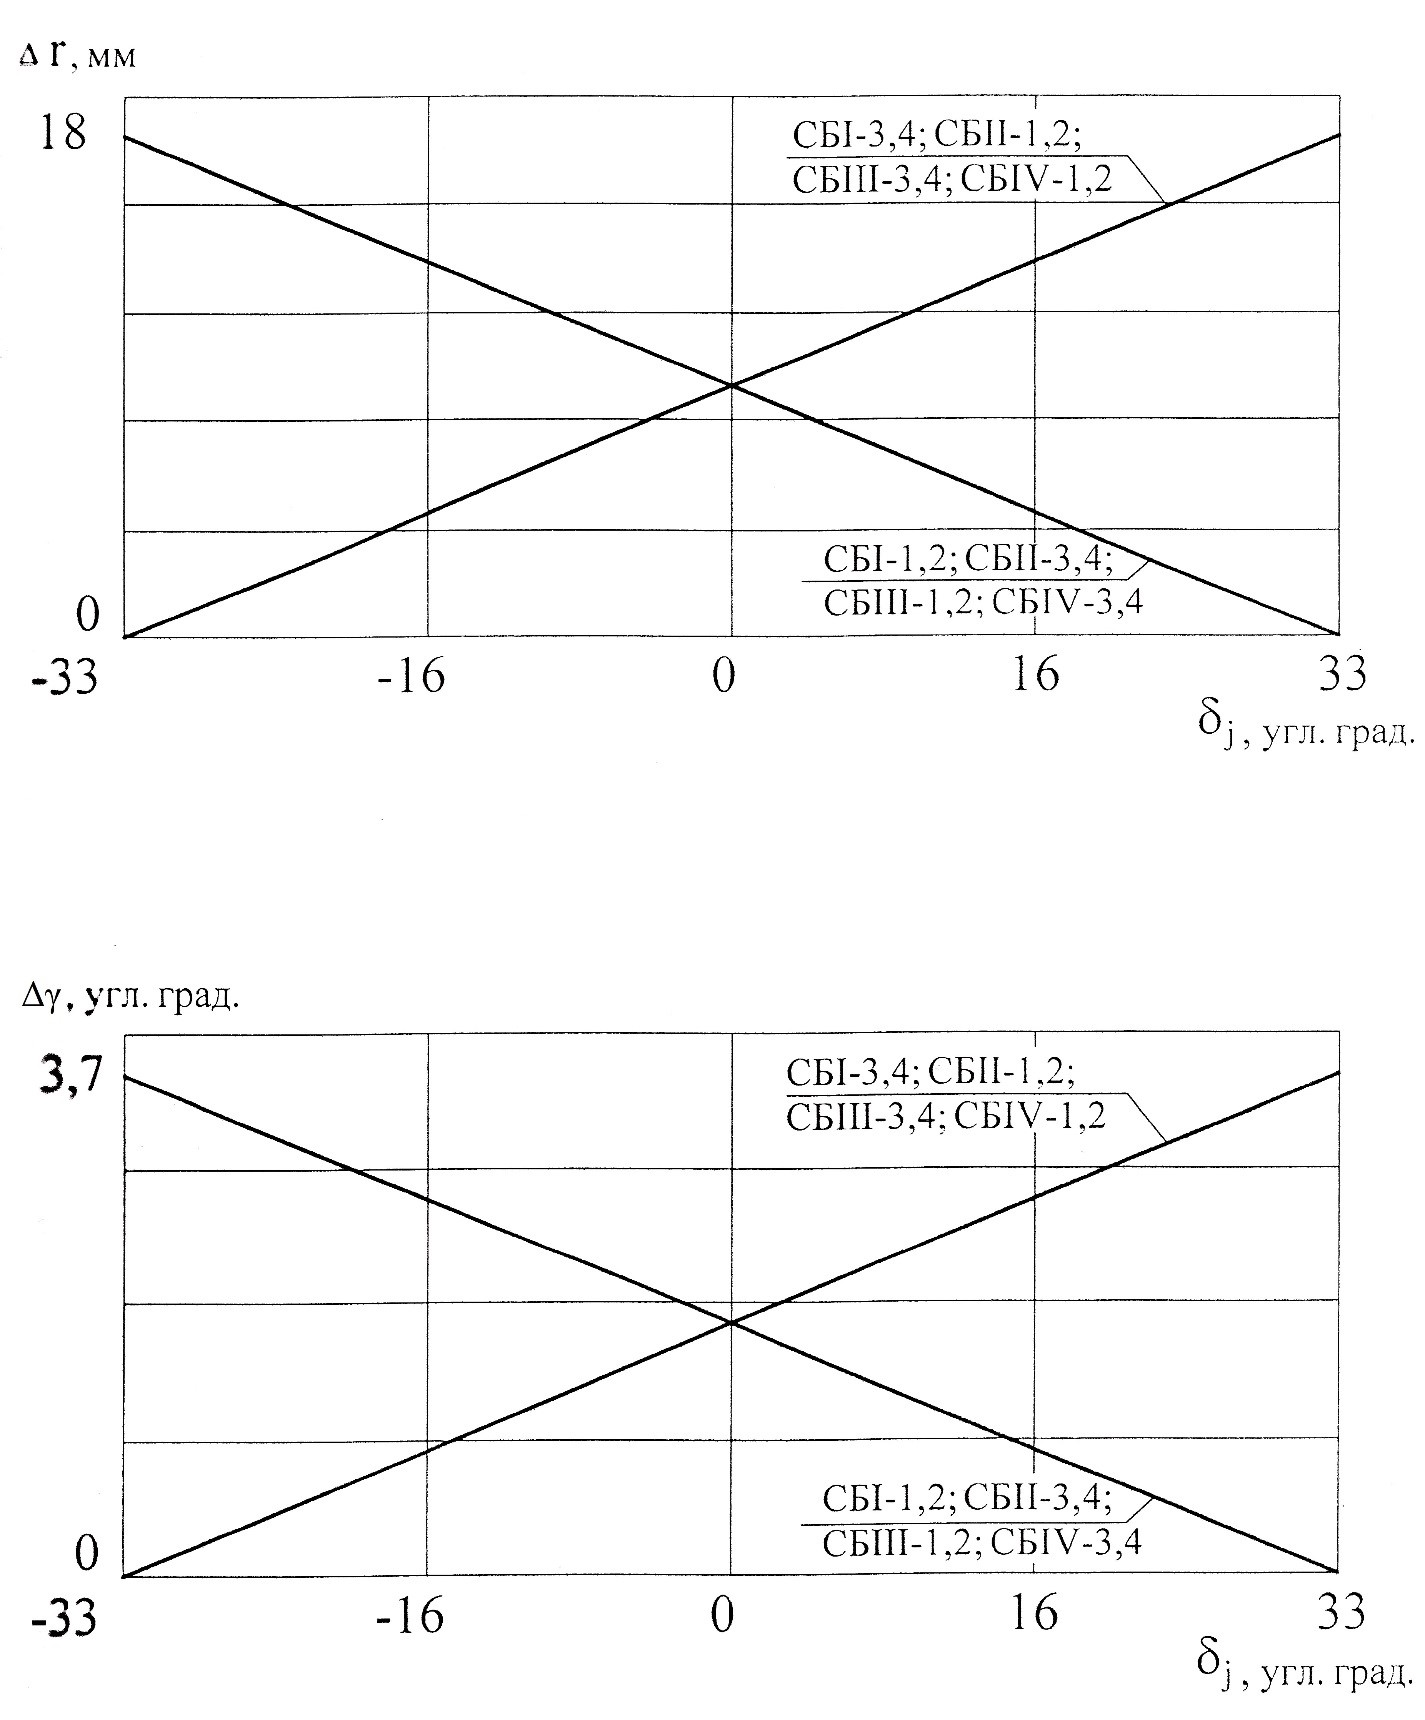
\includegraphics[scale=0.5]{images/linear_vect_draft.jpg}
	\caption{Линейное ($\Delta r$) и угловое ($\Delta \gamma$) отклонение линии действия вектора тяги от геометрической оси сопла в зависимости от угла поворота вала РМ}
	\label{fig:lin_angle_otklonenie}
\end{figure}

\clearpage

\subsection{Требования к СУ}
Исходными данными на разработку технических предложений по алгоритмам СУ, СУ ПТДУ для управления на участке посадки возвращаемого аппарата определены следующие положения:
\begin{itemize}
	\item Начальные условия при запуске ПТДУ:
	\begin{itemize}
		\item угол наклона траектории $-70^{\circ} \div -90^{\circ}$
		\item скорость $80 \div 120 \frac{\text{м}}{\text{с}}$
		\item угол атаки $8^{\circ} \div 20^{\circ} $
		\item угловые скорости до $\pm 50$ угл. град/с по трем углам одновременно
		\item высота $700 \div 1200$ м.
	\end{itemize}
	\item Условия окончания:
	\begin{itemize}
		\item на высоте ~ $20$ м начинается участок вертикального движения, который завершается касанием. Скорость во время касания $2 \div 3 \frac{\text{м}}{\text{с}}$
	\end{itemize}
	\item суммарный импульс тяги:
	$$\int \limits_{0}^T R(r) dt = 280 \ \text{Тс} \cdot c$$
\end{itemize}
\clearpage
	
	%	Алгоритм определения момента включения ПТДУ
	%	Алгоритм определения момента включения ПТДУ
\section{Алгоритм определения момента включения ПТДУ}
Исходя из независимости движений в ортогональных направлениях и приоритете вертикального канала в процессе управления, выбор момента включения ДУ определяется высотой, скоростью движения аппарата и необходимостью обеспечения наиболее предпочтительного режима работы ПТДУ.

Предпочтительным режимом является работа в середине линейного диапазона регулирования тяги, так как при действии возмущений такой режим создает наилучшие условия для управления.

В связи с тем, что аппарат на момент включения ПТДУ движется практически с установившейся скоростью, суммарная потенциальная и кинетическая энергия, которую необходимо рассеять с помощью ПТДУ, убывает при снижении аппарата:

\begin{equation}
E(h) = \frac{mv^2}{2} + mgh
\end{equation}
где $v \ \approx const$

Принимая равенство совершаемой двигателем работы и энергии аппарата, погашаемой на участке спуска при величине тяги двигателя, соответствующей середине диапазона регулирования $E = R_{cp} \eta_0$, получаем высоту включения ПТДУ:

\begin{equation}
\eta_0 = \frac{m v^2}{2} \cdot \frac{1}{R_{cp} + C_x \rho S_m \frac{v^2_\eta}{6} - mg}
\end{equation}
здесь $R_{cp} = 12$Тс.

Этот функционал может вычисляться на борту и при возможном разбросе начальной скорости $v_{\eta_0}$ в пределах $80 \div 120 \frac{\text{м}}{\text{с}}$, высота включения ПТДУ лежит в пределах $\eta_0 = 400 \div 800\text{м}$. 
Предполагая, что в вертикальном канале реализуется движение с постоянным замедлением, т. е. $\Dot{V}_\eta = const$, получаем интегралы движения:
\begin{equation}
\eta = \eta_0 - V_\eta \cdot t + \frac{\Dot{V}_\eta \cdot t^2}{2}
\label{eq:int-eq}
\end{equation}
\begin{equation}
V_\eta = -V_{\eta_0} + \Dot{V}_\eta \cdot t
\end{equation}
откуда
\begin{equation}
\Dot{V}_\eta = \frac{V^2_{\eta_0}}{2 \eta_0}
\label{eq:usk_v_eta}
\end{equation}
\begin{equation}
T = -\frac{V_{\eta_0}}{\Dot{V}_\eta}
\end{equation}

Среднее значение вертикального ускорения, обеспечивающего затормаживание на заданной высоте $\Dot{v}_\eta \approx 12 \div 20 \frac{\text{м}}{\text{с}^2}$, и время торможения $T \approx 8 -10 $с. При этом минимальный суммарный импульс тяги, расходуемый на затормаживание аппарата равен $\approx 150 \text{Тс} \cdot \text{с}$. На участке вертикального спуска расходуется еще $\approx 70 \div 80 \text{Тс} \cdot \text{с}$.

Минимальная высота включения ПТДУ, при которой еще возможно
погасить энергию аппарата $h_0 \approx 400 \text{м}$, время торможения $\approx 7 \text{c}$, тяга $R_{max} = 22 \text{Тс}$. При этом перемещения в горизонтальной плоскости исключаются. Весь импульс при этом сбрасывается в вертикальном канале управления.
\clearpage
	
	%	Математическая модель движения ЦМ ВА
	%	Математическая модель движения ЦМ ВА
\section{Математическая модель движения ЦМ ВА}
Модель движения ЦМ запишем в следующем виде:
\begin{equation}
	\left\{ \begin{matrix}
			\dot{W}_{X1} = \frac{F_{X1}}{m} \\
			\dot{W}_{Y1} = \frac{F_{Y1}}{m} \\
			\dot{W}_{Z1} = \frac{F_{Z1}}{m} \\
		\end{matrix} \right. ,
\end{equation}
где $\dot{W}_{X1}$, $\dot{W}_{Y1}$, $\dot{W}_{z1}$ - проекции кажущегося ускорения на оси связанной системы координат, $F_{X1}$, $F_{Y1}$, $F_{Z1}$ - проекции сил действующих на ВА, $m$ - масса ВА.

\begin{equation}
	\begin{gathered}
		F_{X1} = X - R_{\sum}, \\ 
		F_{Y1} = F_{\text{упр}Y1} + Y, \\
		F_{Z1} = F_{\text{упр}Z1} + Z,
	\end{gathered}
\end{equation}
где $R_{\sum}$ - суммарная сила тяги действующая по оси $OX_1$ связанной системы координат, $F_{\text{упр}Y1}$ - управляющая сила действующая по оси $OY_1$ связанной системы координат, $F_{\text{упр}Z1}$ - управляющая сила действующая по оси $OZ_1$ связанной системы координат, $X$ - продольная составляющая аэродинамической силы, $Y$ - нормальная составляющая аэродинамической силы, $Z$ - поперечная составляющая аэродинамической силы.
\clearpage

\subsection{Расчет управляющих сил}

На ЛА во время полета также действуют управляющие силы и моменты, которые создаются с помощью СУБ

%рисунок направление тяги
Угол наклона сопел равен $\alpha_c = 5.73^{\circ}$ показан на рисунке , максимальная суммарная тяга равна $$R_{max}^{\sum} = 22 \text{Тс}$$

Максимальная тяга $i$ - го сопла $$R_{\max i} = 2.75 \text{Тс}$$

Минимальная суммарная тяга $$R^{\sum}_{\min} = 8 \text{Тс}$$

Минимальная тяга $i$ - го сопла $$R_{\min i} = 1 \text{Тс}$$

\clearpage

\subsection{Расчет аэродинамических сил}
При полете ЛА в атмосфере на них действует сопротивление воздуха, называемое аэродинамическим.

Аэродинамическая сила $R_A$ складывается из сил давления воздуха, направленных по нормалям к поверхности ЛА, и сил трения воздуха касательных к ней. 

Для определения $R_{A}$ используют формулу:
\begin{equation}
	R_{A} = C_{R} \cdot q \cdot S, 
\end{equation}
где $q = \frac{\rho \cdot V^2}{2}$ - скоростной напор набегающего невозмущенного потока, $V$ - скорость набегающего потока, $\rho$ - плотность атмосферы, $S_\text{м}$ - характерная площадь ракеты, $M$ - число маха ракеты, $C_R$ - безразмерный аэродинамический коэффициент, зависящий от формы ракеты.

Запишем формулу для нахождения аэродинамической силы в плоскости $O Y_1 Z_1$:
\begin{equation}
	R_{Y_1 Z_1} = C_{Y1} (\alpha^*, M) \cdot q \cdot S_M
\end{equation}

Продольную составляющую аэродинамической силы запишем следующим образом: 
\begin{equation}
	X = C_{X_1} \cdot q \cdot S_M
\end{equation}

Нормальная составляющая аэродинамической силы:
\begin{equation}
	Y = R_{Y_1 Z_1} \cdot cos \varphi
\end{equation}

Поперечная составляющая аэродинамической силы:
\begin{equation}
	Z = -R_{Y_1 Z_1} sin \varphi
\end{equation}



\clearpage
	
	%	Общая постановка задачи синтеза СУ ПТДУ
	%	Общая постановка задачи синтеза СУ ПТДУ
\section{Общая постановка задачи синтеза СУ ПТДУ}
Исходя из требований ТЗ, при н. у. которые были определены ранее решенной задачей определения момента включения ПТДУ, требуется переместить объект из одной из возможных точек области н. у. в заданную точку пространства (точка зависания) за заданное время. В связи с тем, что органами управления являются не поворачиваемые сопла, т. о. сама задача определяется движением ЦМ и угловым движением. В связи с компоновкой сопловых блоков ВА эти задачи взаимосвязаны. Для того чтобы упростить задачу на данном этапе синтеза будем считать что есть приведенные моменты и приведенные силы. Распределения сил и моментов по соплам это задача следующего этапа. Чтобы синтез управления упростить мы декомпозируем систему на две независимые подсистемы: управления ЦМ и Управления угловым положением на основе разделения движений. Считаем, что динамика требуемой угловой ориентации на порядок быстрее чем движения ЦМ.

При этом каждой из этих подсистем управления выдвигаются свои требования по качеству:
\begin{enumerate}
	\item Время переходного процесса
	\item Осутствие перерегулирования
	\item Точность вывода в точку при вариации н. у. в области, которая ранее была определена алгоритмом включения ПТДУ
\end{enumerate}
\newpage

\subsection{Постановка задачи управления ЦМ}

Цель управления: 
\begin{equation}
|| x(t) - x_{*}(t) || \leq \Delta_x, \  \forall t \geq \hat{t}
\label{eq:ur_target_control}
\end{equation}
где $x(t) = (\xi \ \dot{\xi} \ \eta\  \dot{\eta} \ \zeta \ \dot{\zeta})^T$ - вектор состояния объекта управления относительно центра масс, $x_{*}(t)$ - желаемая траектория спускаемого аппарата с заданными показателями качества.

Это была общая постановка задачи управления. Для того чтобы решить данную задачу мне нужно прежде всего сформировать желаемую траекторию и стабилизироваться относительно 
её.

Таким образом, задача распадается на две подзадачи:
\begin{enumerate}
	\item Синтез желаемой кинематической траектории с учетом желаемой динамики движения по данной траектории.
	\item Стабилизация ЦМ ВА относительно желаемой траектории (задача слежения)
\end{enumerate}
\clearpage
	
	%	Синтез желаемой кинематической траектории
	%	Синтез алгоритмов стабилизации
	%	Заключение
	%	Библиография
\end{document}
	